\documentclass[10pt,a4paper]{article}

% content/resources/templates/preamble.tex
\usepackage[margin=0.6in]{geometry}
\author{Milav Dabgar}
\usepackage{amsmath,amssymb,amsthm}
\usepackage{booktabs}
\usepackage{multirow}
\usepackage{xcolor}
\usepackage{tcolorbox}
\tcbuselibrary{breakable,skins}
\usepackage[colorlinks=true,linkcolor=blue]{hyperref}
\usepackage{titlesec}
\usepackage{enumitem}
\usepackage{tikz}
\usepackage{pgfplots}
\usepackage{circuitikz}
\usepackage[version=4]{mhchem}
\usepackage{longtable}
\usepackage{array}
\usepackage{float}
\usepackage{caption}
\usepackage{listings}

\lstset{
  basicstyle=\small\ttfamily,
  breaklines=true,
  breakatwhitespace=false,
  postbreak=\mbox{\textcolor{red}{$\hookrightarrow$}\space},
  float=false,
  numbers=left,
  numberstyle=\tiny\color{gray},
  numbersep=10pt,
  xleftmargin=2em,
  keywordstyle=\color{blue},
  commentstyle=\color{green!60!black},
  stringstyle=\color{purple},
  backgroundcolor=\color{gray!5},
  showstringspaces=false,
  tabsize=2,
  captionpos=b,
  keepspaces=true,
  columns=flexible
}

\pgfplotsset{compat=1.18}
\usetikzlibrary{shapes,arrows,positioning,calc,patterns,decorations.pathmorphing,decorations.markings,arrows.meta}

% Color scheme
\definecolor{headcolor}{RGB}{0,102,204}
\definecolor{keycolor}{RGB}{220,20,60}
\definecolor{solutioncolor}{RGB}{34,139,34}
\definecolor{mnemoniccolor}{RGB}{148,0,211}
\definecolor{codecolor}{RGB}{0,0,100}

% Spacing
\setlength{\parskip}{3pt}
\setlist[itemize]{nosep}
\setlist[enumerate]{nosep}

% Title formatting
\titleformat{\section}{\Large\bfseries\color{headcolor}}{\thesection}{1em}{}
\titleformat{\subsection}{\large\bfseries\color{headcolor}}{\thesubsection}{1em}{}

% Pandoc tightlist compatibility
\providecommand{\tightlist}{%
  \setlength{\itemsep}{0pt}\setlength{\parskip}{0pt}}

% Pandoc longtable compatibility
\newcounter{none}
\def\thenone{}


% content/resources/templates/english-boxes.tex

% Custom environments
\newtcolorbox{solutionbox}{
 breakable,
 enhanced,
 colback=solutioncolor!5!white,
 colframe=solutioncolor!75!black,
 fonttitle=\bfseries,
 title=Solution
}

\newtcolorbox{solutionboxnobreak}{
 colback=solutioncolor!5!white,
 colframe=solutioncolor!75!black,
 fonttitle=\bfseries,
 title=Solution
}

\newtcolorbox{keyformula}{
 breakable,
 enhanced,
 colback=keycolor!5!white,
 colframe=keycolor!75!black,
 fonttitle=\bfseries,
 title=Key Formula
}

\newtcolorbox{mnemonicboxenv}{
 breakable,
 enhanced,
 colback=mnemoniccolor!5!white,
 colframe=mnemoniccolor!75!black,
 fonttitle=\bfseries,
 title=Mnemonic
}

\newcommand{\mnemonicbox}[1]{%
  \begin{mnemonicboxenv}
    #1
  \end{mnemonicboxenv}
}


\begin{document}

\begin{center}
{\Huge\bfseries\color{headcolor} Mathematics-I Solutions}\\[5pt]
{\LARGE DI01000021 -- Winter 2024}\\[3pt]
{\large Semester 1 Study Material}\\[3pt]
{\normalsize\textit{Detailed Solutions and Explanations}}
\end{center}

\vspace{10pt}

\section*{Question 1 [14 marks]}

\textbf{Fill in the blanks/MCQs using appropriate choice from the given options.}

\subsection*{Q1.1 [1 mark]}
\textbf{$\begin{vmatrix} 5 & 1 \\ 2 & 3 \end{vmatrix} = $ \_\_\_\_\_\_\_}

\begin{solutionbox}
\textbf{Answer}: b. 13

\textbf{Solution}:
For 2×2 determinant $\begin{vmatrix} a & b \\ c & d \end{vmatrix} = ad - bc$

$\begin{vmatrix} 5 & 1 \\ 2 & 3 \end{vmatrix} = (5 \times 3) - (1 \times 2) = 15 - 2 = 13$
\end{solutionbox}

\subsection*{Q1.2 [1 mark]}
\textbf{If $A = \begin{bmatrix} 1 & -2 \\ -3 & 4 \end{bmatrix}$, then $2A = $ \_\_\_\_\_\_\_}

\begin{solutionbox}
\textbf{Answer}: c. $\begin{bmatrix} 2 & -4 \\ -6 & 8 \end{bmatrix}$

\textbf{Solution}:
Scalar multiplication multiplies every element by the scalar.
$2 \times \begin{bmatrix} 1 & -2 \\ -3 & 4 \end{bmatrix} = \begin{bmatrix} 2(1) & 2(-2) \\ 2(-3) & 2(4) \end{bmatrix} = \begin{bmatrix} 2 & -4 \\ -6 & 8 \end{bmatrix}$
\end{solutionbox}

\subsection*{Q1.3 [1 mark]}
\textbf{$\log(xy) = $ \_\_\_\_\_\_\_}

\begin{solutionbox}
\textbf{Answer}: a. $\log x + \log y$

\textbf{Solution}:
Product rule of logarithms: $\log_b(mn) = \log_b(m) + \log_b(n)$
\end{solutionbox}

\subsection*{Q1.4 [1 mark]}
\textbf{The value of $\log_{10} 0.001$ is \_\_\_\_\_\_\_}

\begin{solutionbox}
\textbf{Answer}: d. -3

\textbf{Solution}:
$\log_{10} (0.001) = \log_{10} (10^{-3}) = -3 \log_{10} 10 = -3(1) = -3$
\end{solutionbox}

\subsection*{Q1.5 [1 mark]}
\textbf{If $\sin \theta = \frac{3}{5}$, then $\text{cosec } \theta = $ \_\_\_\_\_\_\_}

\begin{solutionbox}
\textbf{Answer}: b. $\frac{5}{3}$

\textbf{Solution}:
$\text{cosec } \theta$ is the reciprocal of $\sin \theta$.
$\text{cosec } \theta = \frac{1}{\sin \theta} = \frac{1}{3/5} = \frac{5}{3}$
\end{solutionbox}

\subsection*{Q1.6 [1 mark]}
\textbf{The period of $\sin(3x)$ is \_\_\_\_\_\_\_}

\begin{solutionbox}
\textbf{Answer}: b. $2\pi/3$

\textbf{Solution}:
The period of $\sin(bx)$ is $\frac{2\pi}{|b|}$.
Here $b=3$, so period = $2\pi/3$.
\end{solutionbox}

\subsection*{Q1.7 [1 mark]}
\textbf{The value of $\sin^{-1}(\frac{1}{2})$ is \_\_\_\_\_\_\_}

\begin{solutionbox}
\textbf{Answer}: a. $\pi/6$

\textbf{Solution}:
$\sin(\pi/6) = \sin(30^{\circ}) = 1/2$.
Therefore, $\sin^{-1}(1/2) = \pi/6$.
\end{solutionbox}

\subsection*{Q1.8 [1 mark]}
\textbf{The range of $\cos^{-1} x$ is \_\_\_\_\_\_\_}

\begin{solutionbox}
\textbf{Answer}: b. $[0, \pi]$

\textbf{Solution}:
By definition, the principal value range for arccos is $[0, \pi]$.
\end{solutionbox}

\subsection*{Q1.9 [1 mark]}
\textbf{The area of a triangle with vertices $(0,0), (4,0), (0,3)$ is \_\_\_\_\_\_\_}

\begin{solutionbox}
\textbf{Answer}: a. 6

\textbf{Solution}:
Base = 4, Height = 3 (Right angled triangle).
Area = $\frac{1}{2} \times \text{base} \times \text{height} = \frac{1}{2} \times 4 \times 3 = 6$.
\end{solutionbox}

\subsection*{Q1.10 [1 mark]}
\textbf{The distance between points $(1,2)$ and $(4,6)$ is \_\_\_\_\_\_\_}

\begin{solutionbox}
\textbf{Answer}: c. 5

\textbf{Solution}:
Distance formula: $d = \sqrt{(x_2-x_1)^2 + (y_2-y_1)^2}$
$d = \sqrt{(4-1)^2 + (6-2)^2} = \sqrt{3^2 + 4^2} = \sqrt{9+16} = \sqrt{25} = 5$
\end{solutionbox}

\subsection*{Q1.11 [1 mark]}
\textbf{$\lim_{x \to 2} (x^2 + 3) = $ \_\_\_\_\_\_\_}

\begin{solutionbox}
\textbf{Answer}: d. 7

\textbf{Solution}:
Direct substitution: $2^2 + 3 = 4 + 3 = 7$.
\end{solutionbox}

\subsection*{Q1.12 [1 mark]}
\textbf{$\lim_{x \to 0} \frac{\sin x}{x} = $ \_\_\_\_\_\_\_}

\begin{solutionbox}
\textbf{Answer}: a. 1

\textbf{Solution}:
Standard limit identity.
\end{solutionbox}

\subsection*{Q1.13 [1 mark]}
\textbf{If $f(x) = x^3$, then $f'(x) = $ \_\_\_\_\_\_\_}

\begin{solutionbox}
\textbf{Answer}: b. $3x^2$

\textbf{Solution}:
Power rule: $\frac{d}{dx}(x^n) = nx^{n-1}$.
$n=3$, so $3x^{3-1} = 3x^2$.
\end{solutionbox}

\subsection*{Q1.14 [1 mark]}
\textbf{$\int x^2 dx = $ \_\_\_\_\_\_\_}

\begin{solutionbox}
\textbf{Answer}: c. $\frac{x^3}{3} + c$

\textbf{Solution}:
Power rule for integration: $\int x^n dx = \frac{x^{n+1}}{n+1} + c$.
$n=2$, so $\frac{x^{2+1}}{2+1} = \frac{x^3}{3} + c$.
\end{solutionbox}

\section*{Question 2 [14 marks]}

\subsection*{Q2.a [3 marks]}
\textbf{Solve the system of linear equations using Matrix Inversion Method:}
$2x + y = 5$
$3x - 2y = 4$

\begin{solutionbox}
\textbf{Solution}:
System form $AX = B$:
$A = \begin{bmatrix} 2 & 1 \\ 3 & -2 \end{bmatrix}, X = \begin{bmatrix} x \\ y \end{bmatrix}, B = \begin{bmatrix} 5 \\ 4 \end{bmatrix}$

Step 1: Find $|A|$ (Determinant)
$|A| = (2)(-2) - (1)(3) = -4 - 3 = -7$
Since $|A| \neq 0$, inverse exists.

Step 2: Find $A^{-1}$
For $2 \times 2$ matrix $\begin{bmatrix} a & b \\ c & d \end{bmatrix}$, adj $A = \begin{bmatrix} d & -b \\ -c & a \end{bmatrix}$
adj $A = \begin{bmatrix} -2 & -1 \\ -3 & 2 \end{bmatrix}$
$A^{-1} = \frac{1}{|A|} \text{adj} A = \frac{1}{-7} \begin{bmatrix} -2 & -1 \\ -3 & 2 \end{bmatrix} = \begin{bmatrix} 2/7 & 1/7 \\ 3/7 & -2/7 \end{bmatrix}$

Step 3: Solve for $X = A^{-1}B$
$X = \frac{1}{-7} \begin{bmatrix} -2 & -1 \\ -3 & 2 \end{bmatrix} \begin{bmatrix} 5 \\ 4 \end{bmatrix}$
$X = \frac{1}{-7} \begin{bmatrix} (-2)(5) + (-1)(4) \\ (-3)(5) + (2)(4) \end{bmatrix}$
$X = \frac{1}{-7} \begin{bmatrix} -10 - 4 \\ -15 + 8 \end{bmatrix} = \frac{1}{-7} \begin{bmatrix} -14 \\ -7 \end{bmatrix}$
$X = \begin{bmatrix} 2 \\ 1 \end{bmatrix}$

Therefore, $x = 2, y = 1$.
\end{solutionbox}

\subsection*{Q2.b [4 marks]}
\textbf{Prove that $\log(\frac{a^2}{bc}) + \log(\frac{b^2}{ac}) + \log(\frac{c^2}{ab}) = 0$}

\begin{solutionbox}
\textbf{Proof}:
LHS = $\log(\frac{a^2}{bc}) + \log(\frac{b^2}{ac}) + \log(\frac{c^2}{ab})$

Using property $\log m + \log n + \log p = \log(mnp)$:
$= \log \left( \frac{a^2}{bc} \times \frac{b^2}{ac} \times \frac{c^2}{ab} \right)$

Combine numerators and denominators:
$= \log \left( \frac{a^2 \cdot b^2 \cdot c^2}{(bc)(ac)(ab)} \right)$
$= \log \left( \frac{a^2 b^2 c^2}{a^2 b^2 c^2} \right)$

Simplify fraction:
$= \log(1)$

We know $\log(1) = 0$.
$= 0$ = RHS

Hence Proved.
\end{solutionbox}

\subsection*{Q2.c [7 marks]}
\textbf{Draw the graph of $y = \cos x$ for $0 \leq x \leq 2\pi$.}

\begin{solutionbox}
\textbf{Table of values}:
\begin{center}
\begin{tabular}{|c|c|c|c|c|c|}
\hline
$x$ & $0$ & $\pi/2$ & $\pi$ & $3\pi/2$ & $2\pi$ \\
\hline
$y = \cos x$ & $1$ & $0$ & $-1$ & $0$ & $1$ \\
\hline
\end{tabular}
\end{center}

\textbf{Graph}:
\begin{center}
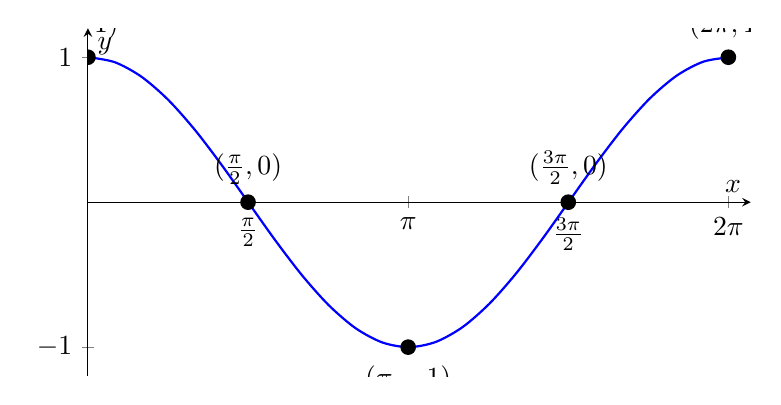
\begin{tikzpicture}
\begin{axis}[
    axis lines=middle,
    xmin=0, xmax=6.5,
    ymin=-1.2, ymax=1.2,
    xtick={0, 1.57, 3.14, 4.71, 6.28},
    xticklabels={$0$, $\frac{\pi}{2}$, $\pi$, $\frac{3\pi}{2}$, $2\pi$},
    ytick={-1, 1},
    xlabel=$x$, ylabel=$y$,
    width=10cm, height=6cm
]
\addplot[smooth, thick, blue, domain=0:6.3] {cos(deg(x))};
\node[label={90:$(0,1)$},circle,fill,inner sep=2pt] at (axis cs:0,1) {};
\node[label={90:$(\frac{\pi}{2},0)$},circle,fill,inner sep=2pt] at (axis cs:1.57,0) {};
\node[label={-90:$(\pi,-1)$},circle,fill,inner sep=2pt] at (axis cs:3.14,-1) {};
\node[label={90:$(\frac{3\pi}{2},0)$},circle,fill,inner sep=2pt] at (axis cs:4.71,0) {};
\node[label={90:$(2\pi,1)$},circle,fill,inner sep=2pt] at (axis cs:6.28,1) {};
\end{axis}
\end{tikzpicture}
\end{center}
\end{solutionbox}

\section*{Question 3 [14 marks]}

\subsection*{Q3.a [3 marks]}
\textbf{Find the value of $\sin(75^{\circ})$.}

\begin{solutionbox}
\textbf{Solution}:
$\sin(75^{\circ}) = \sin(45^{\circ} + 30^{\circ})$

Using identity $\sin(A+B) = \sin A \cos B + \cos A \sin B$:
$= \sin(45^{\circ})\cos(30^{\circ}) + \cos(45^{\circ})\sin(30^{\circ})$

Substitute standard values:
$= \left(\frac{1}{\sqrt{2}}\right)\left(\frac{\sqrt{3}}{2}\right) + \left(\frac{1}{\sqrt{2}}\right)\left(\frac{1}{2}\right)$
$= \frac{\sqrt{3}}{2\sqrt{2}} + \frac{1}{2\sqrt{2}}$
$= \frac{\sqrt{3} + 1}{2\sqrt{2}}$
\end{solutionbox}

\subsection*{Q3.b [4 marks]}
\textbf{Prove that $\frac{1 - \cos A}{\sin A} = \tan(\frac{A}{2})$.}

\begin{solutionbox}
\textbf{Proof}:
LHS = $\frac{1 - \cos A}{\sin A}$

Using half-angle identities:
$1 - \cos A = 2\sin^2(A/2)$
$\sin A = 2\sin(A/2)\cos(A/2)$

Substitute into expression:
$= \frac{2\sin^2(A/2)}{2\sin(A/2)\cos(A/2)}$

Cancel common terms ($2$ and $\sin(A/2)$):
$= \frac{\sin(A/2)}{\cos(A/2)}$
$= \tan(A/2)$
= RHS

Hence Proved.
\end{solutionbox}

\subsection*{Q3.c [7 marks]}
\textbf{Inverse Trigonometry Problem: Prove $\tan^{-1}(\frac{1}{2}) + \tan^{-1}(\frac{1}{3}) = \frac{\pi}{4}$.}

\begin{solutionbox}
\textbf{Proof}:
Using identity $\tan^{-1} x + \tan^{-1} y = \tan^{-1} \left( \frac{x+y}{1-xy} \right)$ if $xy < 1$.

Here $x=1/2, y=1/3$.
$xy = (1/2)(1/3) = 1/6 < 1$. Condition satisfied.

LHS = $\tan^{-1} \left( \frac{1/2 + 1/3}{1 - (1/2)(1/3)} \right)$
Numerator: $1/2 + 1/3 = \frac{3+2}{6} = 5/6$
Denominator: $1 - 1/6 = 5/6$

$= \tan^{-1} \left( \frac{5/6}{5/6} \right)$
$= \tan^{-1}(1)$

Since $\tan(\pi/4) = 1$:
$= \pi/4$
= RHS

Hence Proved.
\end{solutionbox}

\section*{Question 4 [14 marks]}

\subsection*{Q4.a [3 marks]}
\textbf{Find the midpoint of the line segment joining $A(2,3)$ and $B(4,7)$.}

\begin{solutionbox}
\textbf{Solution}:
Midpoint formula $M = \left( \frac{x_1+x_2}{2}, \frac{y_1+y_2}{2} \right)$

$x_1=2, y_1=3$
$x_2=4, y_2=7$

$M = \left( \frac{2+4}{2}, \frac{3+7}{2} \right)$
$M = \left( \frac{6}{2}, \frac{10}{2} \right)$
$M = (3, 5)$
\end{solutionbox}

\subsection*{Q4.b [4 marks]}
\textbf{Find the equation of a line passing through $(2, -1)$ with slope $3$.}

\begin{solutionbox}
\textbf{Solution}:
Point-slope form: $y - y_1 = m(x - x_1)$
Given $m=3, (x_1, y_1) = (2, -1)$.

$y - (-1) = 3(x - 2)$
$y + 1 = 3x - 6$
$y = 3x - 7$ or $3x - y - 7 = 0$
\end{solutionbox}

\subsection*{Q4.c [7 marks]}
\textbf{Evaluate $\lim_{x \to 0} \frac{\sqrt{1+x} - 1}{x}$.}

\begin{solutionbox}
\textbf{Solution}:
Direct substitution yields $0/0$ (Indeterminate form).
Rationalize the numerator:
$= \lim_{x \to 0} \frac{\sqrt{1+x} - 1}{x} \times \frac{\sqrt{1+x} + 1}{\sqrt{1+x} + 1}$
$= \lim_{x \to 0} \frac{(1+x) - 1}{x(\sqrt{1+x} + 1)}$
$= \lim_{x \to 0} \frac{x}{x(\sqrt{1+x} + 1)}$

Cancel x ($x \neq 0$):
$= \lim_{x \to 0} \frac{1}{\sqrt{1+x} + 1}$

Now substitute $x=0$:
$= \frac{1}{\sqrt{1+0} + 1} = \frac{1}{1+1} = \frac{1}{2}$
\end{solutionbox}

\section*{Question 5 [14 marks]}

\subsection*{Q5.a [3 marks]}
\textbf{Differentiate $y = e^x \sin x$ with respect to $x$.}

\begin{solutionbox}
\textbf{Solution}:
Using Product Rule: $(uv)' = u'v + uv'$
Let $u = e^x \Rightarrow u' = e^x$
Let $v = \sin x \Rightarrow v' = \cos x$

$\frac{dy}{dx} = (e^x)(\sin x) + (e^x)(\cos x)$
$\frac{dy}{dx} = e^x(\sin x + \cos x)$
\end{solutionbox}

\subsection*{Q5.b [4 marks]}
\textbf{Evaluate $\int (3x^2 + 4x - 5) dx$.}

\begin{solutionbox}
\textbf{Solution}:
Integrate term by term:
$= \int 3x^2 dx + \int 4x dx - \int 5 dx$
$= 3\frac{x^3}{3} + 4\frac{x^2}{2} - 5x + c$
$= x^3 + 2x^2 - 5x + c$
\end{solutionbox}

\subsection*{Q5.c [7 marks]}
\textbf{Find the maximum and minimum values of $f(x) = x^3 - 3x^2 + 2$ on $[-1, 3]$.}

\begin{solutionbox}
\textbf{Solution}:
Step 1: Find critical points ($f'(x) = 0$).
$f'(x) = 3x^2 - 6x$
$3x(x - 2) = 0 \Rightarrow x = 0, x = 2$
Both points are in $[-1, 3]$.

Step 2: Evaluate $f(x)$ at critical points and endpoints.
Endpoints: $x = -1, x = 3$.

Calculate values:
$f(-1) = (-1)^3 - 3(-1)^2 + 2 = -1 - 3 + 2 = -2$
$f(0) = 0^3 - 3(0)^2 + 2 = 2$
$f(2) = 2^3 - 3(2)^2 + 2 = 8 - 12 + 2 = -2$
$f(3) = 3^3 - 3(3)^2 + 2 = 27 - 27 + 2 = 2$

Maximum Value = 2 (at $x=0$ and $x=3$)
Minimum Value = -2 (at $x=-1$ and $x=2$)
\end{solutionbox}

\vspace{1cm}
\section*{Formula Cheat Sheet}

\begin{keyformula}
\textbf{Logarithms}:
$\log(xy) = \log x + \log y$
$\log(x/y) = \log x - \log y$
$\log(x^n) = n\log x$
\end{keyformula}

\begin{keyformula}
\textbf{Trigonometry}:
$\sin^2 x + \cos^2 x = 1$
$\sin(A+B) = \sin A \cos B + \cos A \sin B$
\end{keyformula}

\begin{keyformula}
\textbf{Differentiation}:
$\frac{d}{dx}(x^n) = nx^{n-1}$
$\frac{d}{dx}(\sin x) = \cos x$
Product Rule: $(uv)' = u'v + uv'$
\end{keyformula}

\end{document}
